\documentclass[12pt,a4paper]{article}
\usepackage{graphicx}
\usepackage{natbib}
\usepackage{float} %dovuto importare questo per poter mettere le figure dove voglio(solo con h! non adava dove volevo)
\usepackage{listings}
\usepackage{acronym}
\usepackage[italian]{babel}
\usepackage{newlfont}
\usepackage{lmodern}
\usepackage{xcolor}
\usepackage{wrapfig}
\usepackage{tabularx}
\definecolor{codegreen}{rgb}{0,0.6,0}
\definecolor{codegray}{rgb}{0.5,0.5,0.5}
\definecolor{codepurple}{rgb}{0.58,0,0.82}
\definecolor{backcolour}{rgb}{0.95,0.95,0.92}

\lstdefinestyle{mystyle}{
    backgroundcolor=\color{backcolour},   
    commentstyle=\color{codegreen},
    keywordstyle=\color{magenta},
    numberstyle=\tiny\color{codegray},
    stringstyle=\color{codepurple},
    basicstyle=\ttfamily\footnotesize,
    breakatwhitespace=false,         
    breaklines=true,                 
    captionpos=b,                    
    keepspaces=true,                 
    numbers=left,                    
    numbersep=5pt,                  
    showspaces=false,                
    showstringspaces=false,
    showtabs=false,                  
    tabsize=2
}

\lstset{style=mystyle}





\title{Introduzione ai Big Data - Monografia}
\author{Emanuele Coltro}
%\subtitle{Strumento per la sostenibilità o Greenwashing}
\begin{document}


% General Setting of listings
\lstset{
  aboveskip=1em,
  breaklines=true,
  abovecaptionskip=-6pt,
  captionpos=b,
  escapeinside={\%*}{*)},
  frame=single,
  numbers=left,
  numbersep=15pt,
  numberstyle=\tiny,
}
% 0. Basic Color Theme
\lstdefinestyle{colored}{ %
  basicstyle=\ttfamily,
  backgroundcolor=\color{white},
  commentstyle=\color{green}\itshape,
  keywordstyle=\color{blue}\bfseries\itshape,
  stringstyle=\color{red},
}
% 1. General Python Keywords List
\lstdefinelanguage{PythonPlus}[]{Python}{
  morekeywords=[1]{,as,assert,nonlocal,with,yield,self,True,False,None,} % Python builtin
  morekeywords=[2]{,__init__,__add__,__mul__,__div__,__sub__,__call__,__getitem__,__setitem__,__eq__,__ne__,__nonzero__,__rmul__,__radd__,__repr__,__str__,__get__,__truediv__,__pow__,__name__,__future__,__all__,}, % magic methods
  morekeywords=[3]{,object,type,isinstance,copy,deepcopy,zip,enumerate,reversed,list,set,len,dict,tuple,range,xrange,append,execfile,real,imag,reduce,str,repr,}, % common functions
  morekeywords=[4]{,Exception,NameError,IndexError,SyntaxError,TypeError,ValueError,OverflowError,ZeroDivisionError,}, % errors
  morekeywords=[5]{,ode,fsolve,sqrt,exp,sin,cos,arctan,arctan2,arccos,pi, array,norm,solve,dot,arange,isscalar,max,sum,flatten,shape,reshape,find,any,all,abs,plot,linspace,legend,quad,polyval,polyfit,hstack,concatenate,vstack,column_stack,empty,zeros,ones,rand,vander,grid,pcolor,eig,eigs,eigvals,svd,qr,tan,det,logspace,roll,min,mean,cumsum,cumprod,diff,vectorize,lstsq,cla,eye,xlabel,ylabel,squeeze,}, % numpy / math
}
% 2. New Language based on Python
\lstdefinelanguage{PyBrIM}[]{PythonPlus}{
  emph={d,E,a,Fc28,Fy,Fu,D,des,supplier,Material,Rectangle,PyElmt},
}
% 3. Extended theme
\lstdefinestyle{colorEX}{
  basicstyle=\ttfamily,
  backgroundcolor=\color{white},
  commentstyle=\color{darkgreen}\slshape,
  keywordstyle=\color{blue}\bfseries\itshape,
  keywordstyle=[2]\color{blue}\bfseries,
  keywordstyle=[3]\color{grass},
  keywordstyle=[4]\color{red},
  keywordstyle=[5]\color{orange},
  stringstyle=\color{darkred},
  emphstyle=\color{pink}\underbar,
}
\sffamily
%\textwidth=450pt\oddsidemargin=0pt
\begin{titlepage}
    \begin{center}
    {{\Large{\textsc{Università Telematica Internazionale Uninettuno}}}} \rule[0.1cm]{14cm}{0.1mm}
    \rule[0.5cm]{14cm}{0.6mm}
    
    
    {\small{\bf INGEGNERIA INFORMATICA \\Corsi di Laurea Magistrale - Big Data\\}}
    \vspace{6mm}
    {\LARGE{\bf Introduzione ai Big Data}}
    
    \end{center}
    \begin{figure}[H]
        \centering
        
\includegraphics[scale=.5]{img/logoUni.png}
    \end{figure}
    \vspace{15mm}
    
    \begin{center}
    {\LARGE{\bf Progetto su R, MapReduce e Hadoop}}\\
    \vspace{3mm}
    {\large{\bf "Contabilità ditta"}}\\
    \vspace{3mm}
    \end{center}
    \vspace{40mm}
    \par
    \noindent
    \begin{minipage}[t]{0.47\textwidth}
    {\large{\bf Docente:\\
    Prof. Pirrone Daniele}}
    \end{minipage}
    \hfill
    \begin{minipage}[t]{0.47\textwidth}\raggedleft
    {\large{\bf Studente:\\
    Emanuele Coltro\\
    }}
    mat: 671HHHINGINFOR
    \end{minipage}
    \vspace{20mm}
    \begin{center}
    {\large{\bf
    Anno Accademico 2022-2023}}%inserire l'anno accademico a cui si Ë iscritti
    \end{center}
    \end{titlepage}
\section*{Abstract}

Il presente paper ha l'obiettivo di esaminare le potenzialità e le performance degli strumenti utilizzati per la gestione e l'analisi dei Big Data. Viene approfondito il processo che porta alla produzione di report grafici, tabelle e schemi a partire dai dati di un problema o di una esigenza. La relazione fornisce informazioni dettagliate su come impostare un progetto, dalla scelta e impostazione dell'ambiente di sviluppo alla contestualizzazione delle decisioni prese. Inoltre, vengono allegati i codici per la generazione dei risultati e dei grafici.

Il progetto in esame mira a soddisfare l'esigenza dell'azienda (fittizzia) STECCAPARAPETUTTI S.R.L. di risolvere un problema di contabilità mediante l'estrazione di alcune feature dai dati. A tal fine, sono stati impiegati strumenti avanzati per l'elaborazione dei dati, tra cui algoritmi di MapReduce e tecniche di visualizzazione avanzata.

L'analisi dei dati è stata eseguita utilizzando il linguaggio R per una prima analisi, seguito dall'utilizzo di un tool scritto in JavaScript per prototipare il sistema di MapReduce e risolvere il problema.
\tableofcontents

\section{Introduzione}
In questa fase, forniremo le basi dei concetti teorici e degli strumenti utilizzati nel corso del progetto. Vedremo in dettaglio come sia stato impostato l'ambiente di sviluppo e come sia stato affrontato il problema in analisi.

\subsection{Richieste}
La società fittizia STECCAPARAPETUTTI S.R.L. richiede l'analisi dei dati delle vendite del sistema di contabilità dell'anno precedente. I dati sono contenuti in un file CSV strutturato in modo omogeneo. L'analisi richiede il calcolo della media e della varianza delle vendite per ogni mese di ogni anno, l'identificazione del mese di ogni anno con la maggiore e minore vendita. Per ogni lavoro, è necessaria la documentazione dell'implementazione in R e dell'implementazione del paradigma MapReduce di Hadoop. Il risultato finale deve essere presentato sotto forma di un rapporto completo.

\subsection{Introduzione all’ambiente}
\subsubsection{MapReduce}
L'algoritmo MapReduce è un modello di programmazione e un'infrastruttura di elaborazione distribuita utilizzata per elaborare e generare informazioni da enormi quantità di dati in modo efficiente, sicuro e scalabile. È stato introdotto da Google\cite{mapReduceGoogle} e ha giocato un ruolo fondamentale nel campo del data processing su larga scala.

L'idea alla base di MapReduce è suddividere un grande task di elaborazione dei dati in due fasi principali: la fase di "map" e la fase di "reduce" (più una fase intermedia totalmente automatizzata):

\begin{itemize}
    \item Durante la fase di MapReduce, i dati di input vengono suddivisi in piccoli frammenti e passati a un insieme di processi paralleli chiamati "mapper". Ogni mapper esegue una funzione di mappatura definita dall'utente che prende in ingresso un dato e produce una serie di coppie chiave-valore intermedie. Queste coppie rappresentano il risultato dell'elaborazione dei dati da parte dei mapper.
    \item Dopo la fase di map, il sistema raggruppa le coppie chiave-valore in base alle chiavi e le ordina nella fase di Shuffle e Sort. Questo è un passaggio cruciale poiché consente ai dati correlati di essere inviati allo stesso processo di "reduce".
    \item In questa fase, il sistema assegna le coppie chiave-valore raggruppate ai processi "reducer". Ogni processo reducer esegue una funzione di riduzione definita dall'utente che agisce sulle coppie chiave-valore correlate e produce i risultati finali dell'elaborazione.
\end{itemize}

\begin{figure}[H]
    \centering
    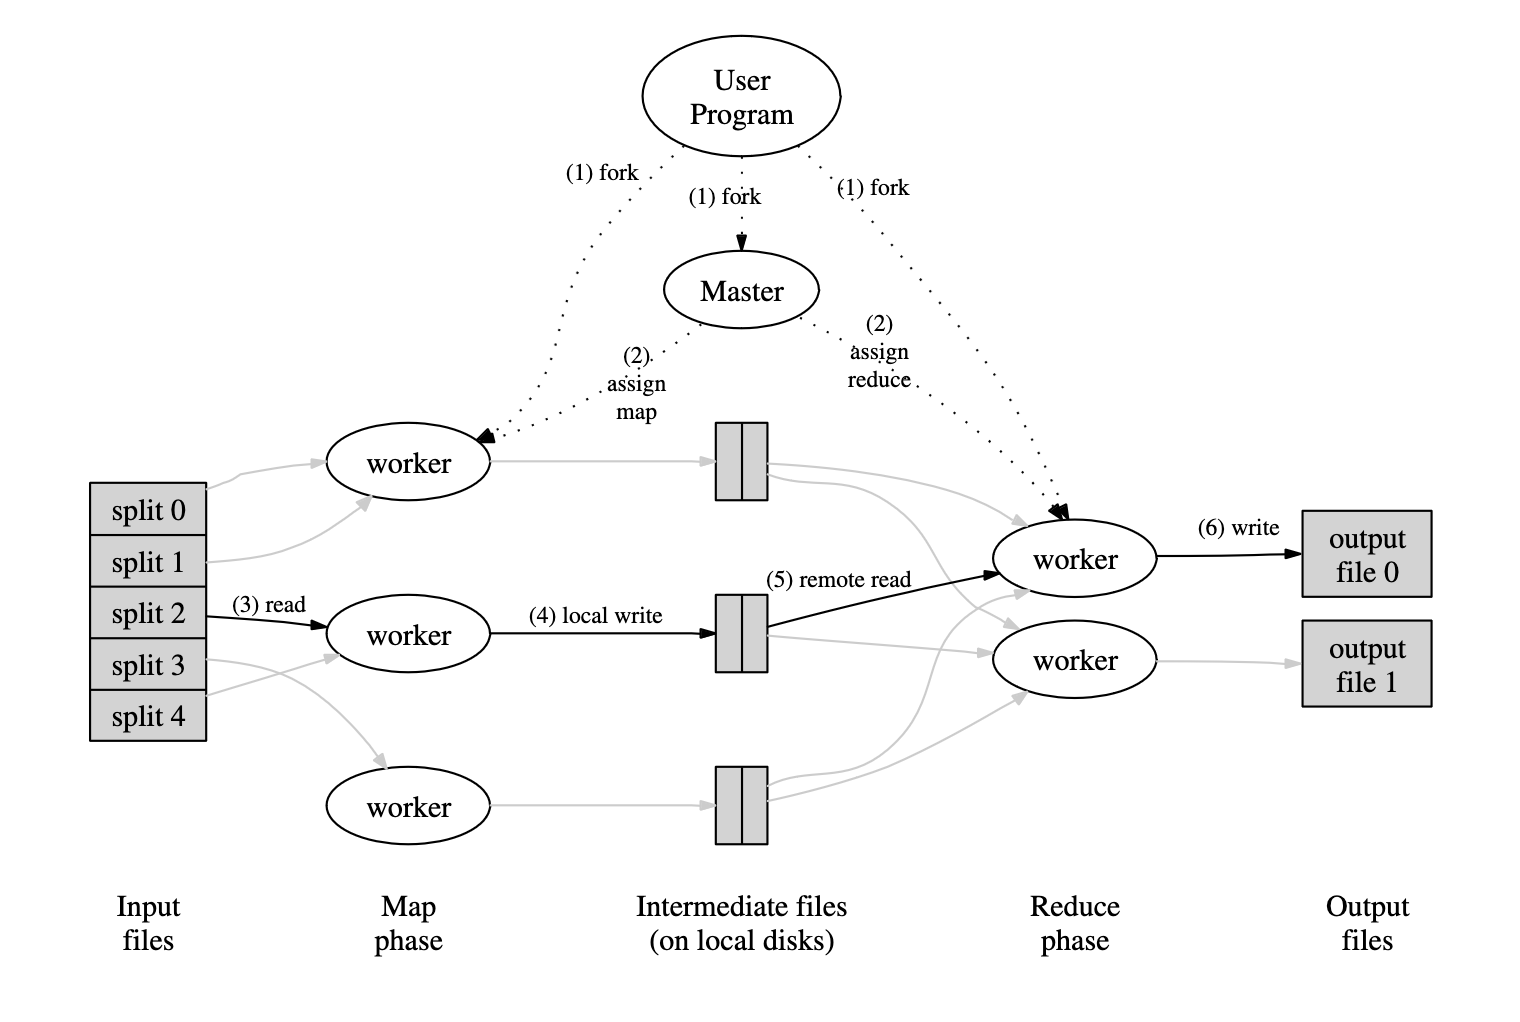
\includegraphics[scale=.4]{img/mapReduceGoogle.png}
    \caption{Schema del processo di MapReduce tratto dal paper di Google}
    \label{mapReduceGoogle}
\end{figure}
L'obiettivo di MapReduce è la parallelizzazione e la distribuzione del carico di lavoro su un cluster di computer, consentendo di elaborare grandi quantità di dati in modo più veloce ed efficiente rispetto a un approccio sequenziale tradizionale. Questo modello di programmazione nasconde molti dettagli complessi dell'elaborazione distribuita, semplificando la creazione di applicazioni che possono sfruttare l'elaborazione su larga scala senza doversi preoccupare delle questioni di basso livello.

Questo ha portato negli anni alla nascita di tecnologie e framework, come Apache Hadoop e Apache Spark, che forniscono funzionalità di MapReduce ma più avanzate e versatili per l'elaborazione distribuita dei dati.

\subsubsection{Hadoop}
Apache Hadoop è un framework open-source sviluppato per consentire l'elaborazione distribuita di grandi quantità di dati su cluster di computer. È basato sulla paper originale di Google su MapReduce e il file system distribuito Google File System (GFS). Hadoop è progettato per gestire l'elaborazione di dati in parallelo su macchine commodity (hardware relativamente economico e accessibile).

Il cuore di Hadoop\cite{ApacheHadoopSite} è composto da due componenti principali: Hadoop Distributed File System (HDFS) e il framework di elaborazione MapReduce.

\begin{enumerate}
    \item Hadoop Distributed File System (HDFS): HDFS è il sistema di archiviazione distribuito di Hadoop. Si basa su un modello di architettura master-slave in cui un nodo master, chiamato "NameNode", gestisce i metadati del file system e tiene traccia di dove sono archiviati i dati. I nodi slave, chiamati "DataNode", contengono i blocchi di dati reali. I dati vengono suddivisi in blocchi e replicati su vari DataNode per garantire la disponibilità e l'affidabilità.
    \begin{figure}[H]
        \centering
        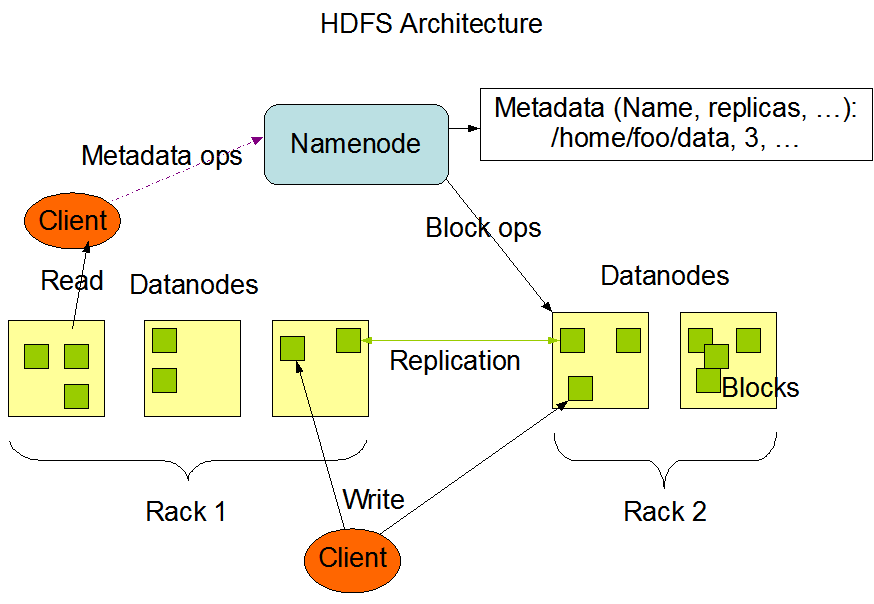
\includegraphics[scale=.4]{img/hdfsarchitecture.png}
        \caption{Schema dell'architettura HDFS tratto dal sito di Hadoop}
        \label{hdfsarchitecture}
    \end{figure}
    \item MapReduce: Come descritto in precedenza, MapReduce è un modello di programmazione per l'elaborazione distribuita. Hadoop implementa questo modello consentendo agli sviluppatori di scrivere programmi MapReduce per l'elaborazione dei dati su cluster. Il framework si occupa della distribuzione delle attività di map e reduce su diversi nodi del cluster, dell'ordinamento e dell'aggregazione dei risultati intermedi e della gestione dei fallimenti dei nodi.
\end{enumerate}

I punti di forza di Hadoop includono la scalabilità orizzontale, la tolleranza ai guasti, l'economia hardware, l'ecosistema di strumenti, l'elaborazione su larga scala, la flessibilità nei tipi di dati e l'elaborazione di dati grezzi. Tuttavia, Hadoop ha anche alcuni svantaggi come la complessità nella configurazione e gestione di un cluster, la latenza, la memoria limitata, l'approccio orientato ai batch, la complessità della programmazione e la concorrenza da parte di framework alternativi come Apache Spark.
\subsubsection{R e RStudio}
R è un linguaggio di programmazione e un ambiente di sviluppo utilizzati principalmente per l’analisi statistica e la visualizzazione dei dati, progettato per lavorare con dataset di varie dimensioni e complessità. Offre un'ampia gamma di funzioni statistiche, algoritmi e pacchetti per l'analisi dei dati, il machine learning, l'analisi delle serie temporali e altro ancora. Inoltre, R fornisce potenti strumenti di visualizzazione che consentono di creare grafici e grafici per rappresentare i dati in modo efficace.

RStudio è un ambiente di sviluppo integrato (IDE) progettato specificamente per lavorare con il linguaggio di programmazione R. Come R\cite{installR} anche RStudio\cite{installRstudio} è un progetto open source che ha lo scopo di offrire un'interfaccia utente intuitiva e ben organizzata che semplifica la scrittura del codice R, l'analisi dei dati e la creazione di visualizzazioni.

\subsubsection{Python}
Python\cite{installPython} è un linguaggio di programmazione che ha catturato l'attenzione di sviluppatori di tutto il mondo grazie alla sua natura versatile e alla sua sintassi chiara e leggibile. Creato da Guido van Rossum\cite{wikiPython} e presentato nel lontano 1991, Python ha continuato a guadagnare popolarità nel corso degli anni, diventando uno dei linguaggi più utilizzati e apprezzati nella comunità dello sviluppo software.

Ciò che distingue Python è il suo approccio alla scrittura del codice. La sua sintassi è strutturata in modo simile al linguaggio naturale, rendendo il codice scritto in Python quasi come una conversazione tra lo sviluppatore e la macchina. Questa semplicità e leggibilità non solo agevolano la creazione del codice, ma anche la comprensione dello stesso da parte di altri sviluppatori, favorendo una collaborazione più agevole.

Python (come anche R) è un linguaggio interpretato, il che significa che non richiede una fase di compilazione separata. Questo aspetto favorisce un approccio di sviluppo più rapido e interattivo, consentendo agli sviluppatori di scrivere e testare il codice in modo immediato, senza dover attendere processi di compilazione lungo.
\subsubsection{Tool Javascript-html per MapReduce}
Per evitare possibili complicazioni dovute alla configurazione di Hadoop, il Professore Daniele Pirrone ha creato uno script web chiamato "Tool MapReduce". Questo strumento consente di simulare un programma MapReduce attraverso un browser generico su Internet.

Lo strumento è sviluppato in Javascript con interfaccia HTML, rendendolo compatibile con i principali sistemi operativi e browser. Il codice è rilasciato sotto licenza GPL.

Lo strumento è semplicemente uno strumento didattico di supporto per gli studenti e quindi:
\begin{itemize}
    \item Consente l'utilizzo di file di input che sono limitati in dimensione alla capacità del computer su cui viene eseguito.
    \item Accetta solo file di testo come input (la maggior parte dei quali hanno un'estensione .txt).
    \item Simula il paradigma di programmazione parallela MapReduce, ma in realtà funziona in modalità stand-alone, non distribuita.
\end{itemize}


\subsection{Preparazione dell’ambiente}
Affrontiamo ora il processo di installazione e configurazione dell'ambiente di sviluppo su macchina virtuale, che si è rivelato necessario per una corretta comunicazione tra Hadoop, RStudio e Python.

Le principali motivazioni di questa scelta risiedono nel fatto che i packages di RHadoop per una corretta comunicazione tra RStudio e Hadoop non sono aggiornati alle ultime versioni (l’ultima release di RHadoop risale al 2015).

La scelta di utilizzare la versione di Hadoop all'interno di una macchina virtuale anziché installarla direttamente sul sistema locale è stata influenzata da problematiche di gestione del DFS estendendo tutto il disco a HDFS andando quindi a creare conflitti.

Sfruttando il contesto isolato che offre la virtualizzazione si ha potuti sperimentare con un approccio trial and error diverse configurazioni che permettessero il corretto funzionamento di tutte le componenti. Sono state così fatte scelte specifiche per quanto riguarda le versioni dle sistema operativo e dei software da utilizzare, tenendo conto della compatibilità tra di essi e delle raccomandazioni della comunità.

Si è scelto Virtualbox come sistema di virtualizzazione in quanto software open source di ampia distribuzione.
\subsubsection{Preparazione dell'ambiente virtuale}
Il primo passo è stato creare una nuova macchina virtuale su VirtualBox dal sistema host (macOs Ventura 13.4 con 2,3 GHz Intel Core i5 dual-core e 16 GB 2133 MHz LPDDR3) assegnando risorse hardware adeguate.
\begin{table}[ht]
\centering
\begin{tabularx}{\textwidth}{|X|X|X|X|X|}
\hline
Ruolo & Sistema Operativo & CPU & RAM & Spazio su disco \\
\hline
Host & macOS Ventura 13.4 & 2.3 GHz Intel Core i5 dual-core & 16 GB 2133 MHz LPDDR3 & 500 GB \\
\hline
VM & Ubuntu 16.04 & 1 CPU & 4 GB & 80 GB \\
\hline
\end{tabularx}
\caption{Specifiche di sistema}
\label{tab:specifiche}
\end{table}
    
È stata scelta una distribuzione Linux (Ubuntu 16.04) come sistema operativo ospite per sfruttare la flessibilità e le prestazioni offerte da questa piattaforma open source. Essendo infatti Apache Hadoop un sistema utilizzato principalmente lato server, la sua implementazione più diffusa e stabile è in ambiente UNIX.
\subsubsection{Installazione di Hadoop}
Per garanzie di compatibilità si è scelto la versione 2.6.5 di Apache Hadoop, andandolo a configurare in modalità Single Node Cluster. Successivamente si è anche cercato di aggiungere nodi al cluster ma con risultati poco stabili.\footnote{In una configurazione iniziale si era utilizzata sia una soluzione "fisica" con due Raspberry Pi 3 Model B come nodi dati, sia macchine virtuali Ubuntu Server 22.04. Entrambe le soluzioni hanno presentato problematiche, quindi si è preferito tornare alla configurazione Single Node.}
\subsubsection{Integrazione di RStudio}
L'integrazione di RStudio è stata relativamente più semplice utilizzando la versione 1.0.153 del 2017 e versione di R 3.2.3 che ha permesso una installazione delle librerie di RHadoop senza conflitti.
\subsubsection{Configurazione di Python}
La configurazione di Python presente già nel sistema operativo offre le versioni 2.7 e 3.5.2 con i relativi comandi python e python3. L’unica configurazione necessaria è stata l’intallazione del gestore di pacchetti Python “pip” per l’installazione delle librerie utilizzate poi negli script.

L'installazione e la configurazione dell'ambiente di sviluppo su VirtualBox con Hadoop, RStudio e Python hanno richiesto un approccio meticoloso e la risoluzione di diverse sfide tecniche. Le scelte fatte durante il processo sono state guidate dalla necessità di garantire l'integrazione corretta dei componenti e l'ottimizzazione delle risorse disponibili.



\section{Conclusioni}
In questo paper abbiamo visto come l'analisi dei dati sia un processo fondamentale per l'ottimizzazione di qualsiasi attività. Attraverso l'analisi di un dataset relativo al fatturato di un'azienda abbiamo mostrato come sia possibile utilizzare gli strumenti più efficaci per la comprensione dei dati.

In particolare, abbiamo utilizzato R come strumento di analisi dei dati e JavaScript, Hadoop e R per l'implementazione di algoritmi di mapreduce. Grazie all'utilizzo di R, abbiamo creato grafici chiari ed efficaci per la comprensione dei dati, come grafici lineari, box plot e grafici a barre con grafico a torta.

Abbiamo anche illustrato il processo di data science, partendo dall'analisi del problema e del dataset, passando per l'elaborazione di algoritmi di mapreduce fino alla produzione di grafici per rispondere alle necessità del problema iniziale.

Inoltre, abbiamo visto come lo strumento di JavaScript per l'implementazione di algoritmi di mapreduce sia un ottimo strumento didattico per approcciarsi al paradigma di programmazione di mapreduce, soprattutto per chi è alle prime armi e non conosce R o Python. Tuttavia, l'utilizzo di Hadoop come software open source è risultato alquanto complicato da configurare correttamente, soprattutto se si vuole andare ad aggiungere nodi al cluster.

In conclusione, abbiamo apprezzato la possibilità di scalare la propria potenza di calcolo e parallelizzare le informazioni, abbiamo visto come la scelta del linguaggio e delle strategie di implementazione di un algoritmo possano incidere sulle performance e di conseguenza sui costi computazionali di un processo.

La gestione di grandi quantità di dati è una disciplina cruciale in un mondo in cui i dati sono sempre più presenti e utilizzati. Gli strumenti e le metodologie utilizzati in questo documento rappresentano i principi base per l'approccio a questa materia, evidenziando come sia necessario adattarsi alle diverse problematiche proposte.
\section*{Allegato 1}
\addcontentsline{toc}{section}{\protect\numberline{}Allegato 1}
\subsection*{Fattori di standardizzazione in base alle tematiche}
\subsubsection*{Energia Primaria}

\lstinputlisting[language=Python, firstline=1, lastline=30, caption=Python exampl]{demo.py}

\lstinputlisting[language=R, firstline=1, lastline=30]{HW_R.r}


Questo indicatore considera la richiesta di energia primaria per l'intero ciclo di vita del prodotto considerato, tenendo conto, ad esempio, della trasformazione dei materiali combustibili in energia elettrica.

A questo indicatore contribuiscono quindi i materiali combustibili con il loro contenuto di energia primaria.

Il fattore di caratterizzazione è in questo caso il potere calorifico del materiale considerato.
\subsubsection*{Effetto Serra}
L'indicatore effetto serra viene calcolato considerando, tra le sostanze emesse in aria, quelle che contribuiscono al potenziale riscaldamento globale del pianeta Terra.

La quantità in massa di ciascuna sostanza, calcolata sull'intero ciclo di vita del prodotto, viene moltiplicata per un coefficiente di peso chiamato potenziale di riscaldamento globale (GWP, Global Warming Potential). Sommando poi i contributi delle varie sostanze, si ottiene il valore aggregato dell'indicatore.

Le sostanze che contribuiscono all'effetto serra sono principalmente: CO2, CH4, N2O, CFC, gli HCFC e gli HFC.

La CO2 è la sostanza di riferimento per questo indicatore, vale a dire che il suo coefficiente di peso è uguale a 1 e i valori dell'indicatore sono espressi in kg di CO2 equivalente (kg CO2 eq).
\begin{table}[!ht]
    \centering
    \begin{tabular}{|| c | c | c ||} %l=left, c=center, r=right il | serve per separare le colonne
        \hline
        \textbf{Composto} &\textbf{Formula	GWP100} & \textbf{[kg CO2/kg gas]}\\
        \hline\hline
        Diossido di carbonio &	CO2	& 1 \\
        \hline
        Ossido di carbonio & CO &	2\\
        \hline
        Metano	& CH4	& 11\\
        \hline
        Ossido di azoto	& N2O	& 320\\
        \hline
        CFC-11	& CFCl3	& 4.000\\
        \hline
        CFC-12	& CF2Cl2	& 8.500\\
        \hline
        Clorotrifluorometano (CFC-13)	& CF3Cl	& 11.700\\
        \hline
        Tetrafluorometano (CFC-14)	& CF4	& 9.300\\
        \hline
        HCFC-22	& CHF2Cl	& 1.700\\
        \hline
        HCFC-125	& CHF2CF3	& 3400\\
        \hline
        Halon-1301	& CF3Br	& 5.600\\
        \hline
        Diclorometano	& CH2Cl2	& 25\\
        \hline
        Cloroformio	& CHCl3	& 15\\
        \hline
    \end{tabular}
    \caption{Fattori di standardizzazione per i principali responsabili dell'effetto serra, basati sul loro diretto contributo al riscaldamento globale con un tempo-orizzonte di 100 anni.}
    \label{tabellaFattoriEffettoSerra}
\end{table}
	 


\subsubsection*{Assottigliamento della fascia di ozono stratosferico}
La riduzione della fascia di ozono stratosferico viene calcolata come l'indicatore precedente, ma utilizzando diverse sostanze (CFC, HCFC) e un diverso coefficiente di peso, chiamato potenziale di riduzione dell'ozono (ODP, Ozone Depletion Potential).

La sostanza di riferimento in questo caso è un clorofluorocarburo, precisamente il CFC-11.
\subsubsection*{Eutrofizzazione}
Questo indicatore valuta l'effetto dell'eutrofizzazione, ovvero l'aumento della concentrazione di sostanze nutritive negli ambienti acquatici. Le sostanze che contribuiscono al fenomeno dell'eutrofizzazione sono i composti a base di fosforo e azoto.

La sostanza di riferimento è il fosfato (PO4) e il coefficiente di peso prende il nome di potenziale di nutrificazione (NP, Nutrification Potential).
\begin{table}[!ht]
    \centering
    \begin{tabular}{|| c | c ||} %l=left, c=center, r=right il | serve per separare le colonne
        \hline
        \textbf{Formula} &\textbf{NEP [kg NO3-/kg compost]} \\
        \hline\hline
        NO3-	& 1\\
        \hline
        NO2	&1.35\\
        \hline
        NOx	& 1.35\\
        \hline
        NO	&2.07\\
        \hline
        N2O	&2.82\\
        \hline
        NH3	&3.64\\
        \hline
        HCN	&2.29\\
        \hline
        N	&4.43\\
        \hline
        PO4---	&10.45\\
        \hline
        P	&32.03\\
        \hline
    \end{tabular}
    \caption{Fattori di standardizzazione per i principali responsabili dell'effetto serra, basati sul loro diretto contributo al riscaldamento globale con un tempo-orizzonte di 100 anni.}
    \label{tabellaFattoriEutrofizzazione}
\end{table}
	

\subsubsection*{Formazione di smog fotochimico (photo-smog)}
Il termine "smog estivo" si riferisce a tutte le sostanze organiche volatili che portano alla formazione di ozono troposferico attraverso reazioni fotochimiche (in presenza di radiazione solare).

Il fattore di caratterizzazione utilizzato è chiamato "potenziale di formazione di ozono fotochimico" (POCP, Photochemical Ozone Creation Potential) e la sostanza di riferimento è l'etilene (C2H4).
\begin{table}[!ht]
    \centering
    \begin{tabular}{|| c | c ||} %l=left, c=center, r=right il | serve per separare le colonne
        \hline
        \textbf{Composto} &\textbf{POCP [g C2H4/g di composto]} \\
        \hline\hline
        metano	&0,007\\
        \hline
        etano	&0,100\\
        \hline
        propano	&0,500\\
        \hline
        aldeidi	&0,3±0,2\\
        \hline
        CO	&0,040\\
        \hline
        metanolo	&0,123\\
        \hline
        etanolo	&0,268\\
        \hline
    \end{tabular}
    \caption{Fattori di standardizzazione per i principali responsabili dello smog fotochimico.}
    \label{tabellaFattoriPhotoSmog}
\end{table}
	

\subsubsection*{Rifiuti Solidi}
L'indicatore in questione raggruppa tutti i rifiuti di tipo solido generati in qualsiasi attività nel ciclo di vita di un prodotto, ad esempio durante la generazione di energia elettrica necessaria per una lavorazione o durante la produzione delle lamiere di acciaio.

Non esistono fattori di caratterizzazione per questo indicatore, e ogni sostanza viene sommata alle altre tenendo semplicemente conto della quantità emessa in massa.

% ativo la parte sotto nel momento in cui faccio delle citazioni
\newpage
\listoffigures
\bibliographystyle{plain}
\bibliography{ref} 
\end{document}